\section{Experiments}

In this section, we conduct corresponding experiments on the D4RL benchmark \cite{fuD4RLDatasetsDeep2021} and the real-world recommendation system scenarios datasets based on RecSim \cite{ieRecSimConfigurableSimulation2019}. Our primary points of comparison are reward modification strategies include: scale, return min-max, average, ensemble. Furthermore, these strategies can be combined with any offline RL algorithms without extra efforts, model-free offline RL algorithms BC, CQL \cite{kumarConservativeQLearningOffline2020} and model-based algorithm MOPO \cite{yuMOPOModelbasedOffline2020} are included depend on the environment as follows:

\begin{itemize}
    \item Behaviour Cloning(BC). BC uses supervised learning for policy learning, and the learning process does not depend on the rewards. Therefore, delaying the rewards has no effect on its policy learning process. In this part, we directly quote the results published in the D4RL paper.

    \item Conservative Q-Learning(CQL). CQL is a type of model-free algorithm  tries to learn a "Conservative" Q-value function by incorporating random samples from state-action distributions, thereby avoiding action out of distribution(OOD) caused by offline Q-Learning.

    \item Model-based Offline Policy Optimization(MOPO). MOPO is a model-based algorithm. It first learns multiple supervised learning models (including state transition and reward function) from offline data, and the strategy interacts with the learned model. The reward adds an additional transition to the joint model. Deterministic estimation, as an empirical reward lower bound, has verified its effectiveness in theory and experiment.

\end{itemize}

We verify the effectiveness of aforementioned methods in solving the delayed rewards problems. Experiments conducted both on simuated offline datasets (OpenAI Gym) and customized real-world datasets. All tasks involves  high-dimensional observation spaces, the delayed rewards introduces extra difficulty for learning effective control strategies in offline setting.

\subsection{Evaluation on D4RL public datasets}

We evaluate our methods together with prior offline RL algorithms on three continuous control tasks from the D4RL bechmark. As the rewards in original datasets are not delayed, we first construct the delay rewards datasets from the none-delayed rewards datasets.

\textbf{Datasets construction.} Without dedicating extra efforts collecting data by training an agent from scratch, we directly delay the original rewards by performing the constant delay transformation: we first set a hyper-parameter $K$ as the delay interval which controls the sparsity of the delayed rewards, the delayed rewards are then computed at equal intervals with $K$ as the un-discounted cumulative rewards of corresponding interval, the missing rewards are filled with 0.
Formally, for a trajectory $\tau = \left(s_0, a_0, r_0, \cdots, s_T, a_t, r_T\right)$, the delayed reward at time step $t$ is defined as $r_t^{delay}$, where:

$$
    \begin{aligned}
        r_t^{delay} = \begin{cases}
            0,                          & \left(t + 1\right) \% K \neq 0; \\
            \sum_{i = t - K + 1}^t r_i, & \text{otherwise}.
        \end{cases}
    \end{aligned}
$$

The transformation above introduces sparsity to delay rewards, meanwhile, it keeps the rule that for any trajectory in the original datasets, the un-discounted cumulative rewards keep constant before and after the operation, mathematically, we have:

$$
    \sum_{t = 0}^{T} r_t = \sum_{t = 0}^{T} r_t^{delay}
$$

The comparison between the immediate rewards and delayed rewards are shown in Figure \ref{fig:fig1}, the immediate rewards are more continuous in scale and dense in spatiality.
\begin{figure}[H]
    \centering
    \begin{subfigure}{0.33\textwidth}
        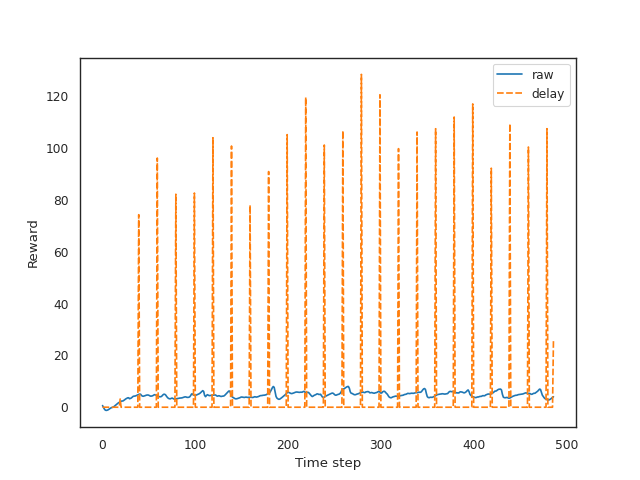
\includegraphics[width=\textwidth]{assets/delay_mode-constant-delay-20_0_delayed.png}
        \caption{Episode rewards}
    \end{subfigure}
    ~
    \begin{subfigure}{0.31\textwidth}
        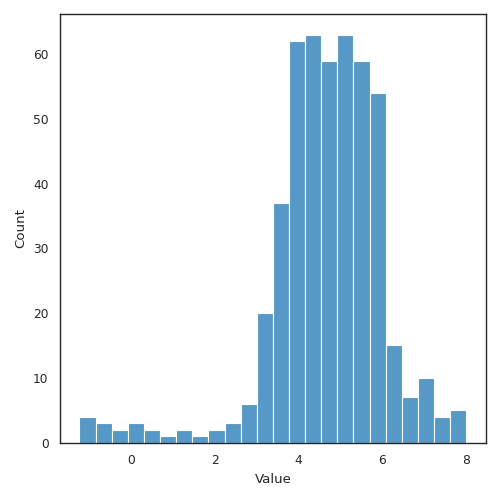
\includegraphics[width=\textwidth]{assets/delay_mode-constant-delay-20_distribution_raw_0_delayed.png}
        \caption{Raw rewards distribution}
    \end{subfigure}
    ~
    \begin{subfigure}{0.31\textwidth}
        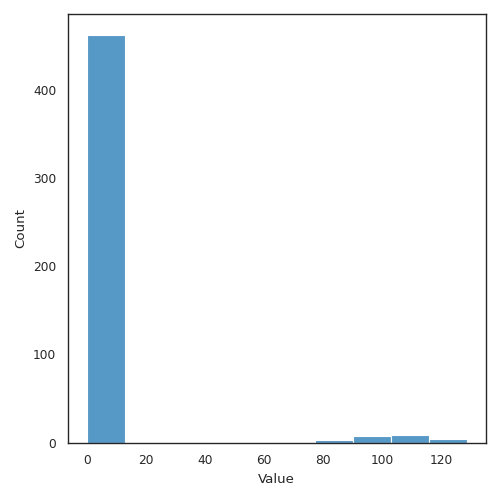
\includegraphics[width=\textwidth]{assets/delay_mode-constant-delay-20_distribution_delay_0_delayed.png}
        \caption{Delay rewards distribution}
    \end{subfigure}
    \caption{Illustrations of immediate rewards and delayed rewards on Walker2d-expert-v0 with delay interval 20. \textbf{Left:} The lineplot of immediate rewards and delayed rewards for a trajectory
        , the blue line denoted as \textit{raw} is the raw immediate rewards, the delayed rewards are drawn in orange. \textbf{Center:} The distribution of the immediate rewards ranges in $\left[-2, 10\right]$.
        \textbf{Right:} The sparse distribution for delayed rewards, In all data samples, about $95\%$ of the samples get reward 0, and the remaining data contains non-zero reward signals and these non-zero rewards are relatively large in value and distributed very scattered.}
    \label{fig:fig1}
\end{figure}


We compare to BC, CQL, and MOPO on Gym domain tasks. The performance of BC has
nothing to do with the setting of delayed rewards, as it directly learns the
policy that maps from observation space to action space, we report the numbers of BC from the original D4RL paper. The policy learning process of CQL and MOPO are strictly bound to the rewards, we run these algorithms based on the
open source reproducing code base \textbf{OfflineRL} published by \citeauthor{qinNeoRLRealWorldBenchmark2021}
on NeoRL paper. Our results are shown in Table \ref{tbl:mujoco_results}.


\begin{table*}[h]
    \centering
    \begin{tabular}{lll|cc|cccc}
        \toprule
                                        &                                     &                                &                            &                              & \multicolumn{4}{c}{\bf MOPO}                                                                                                             \\
        \multicolumn{1}{l}{\bf Dataset} & \multicolumn{1}{c}{\bf Environment} & \multicolumn{1}{c|}{\bf Delay} & \multicolumn{1}{c}{\bf BC} & \multicolumn{1}{c|}{\bf CQL} & \multicolumn{1}{c}{\bf{Normal}} & \multicolumn{1}{c}{\bf +Average} & \multicolumn{1}{c}{\bf +Ensemble} & \multicolumn{1}{c}{\bf +Minmax} \\
        \midrule
        Random                          & HalfCheetah                         & 20                             & $2.1$                      & -                            & $0.1$                           & $\bf{25.3 \pm 1.5 }$                                                                                   \\
        Random                          & Hopper                              & 20                             & $1.6$                      & -                            & $3.1$                           & $\bf{9.1 \pm 1.5 }$                                                                                    \\
        Random                          & Walker2d                            & 20                             & $9.8$                      & -                            & $0.1$                           & $\bf{12.6 \pm 6.1 }$                                                                                   \\
        \midrule
        Medium                          & HalfCheetah                         & 20                             & $36.1$                     & -                            & $-0.8$                          & $\bf{48.3 \pm 2.4}$                                                                                    \\
        Medium                          & Hopper                              & 20                             & $29$                       & -                            & $5.1$                           & $19.0 \pm 8.1$                                                                                         \\
        Medium                          & Walker2d                            & 20                             & $6.6$                      & -                            & $4.5$                           & $\bf{72.3 \pm 0.9}$                                                                                    \\
        \midrule
        Medium-Replay                   & HalfCheetah                         & 20                             & $38.4$                     & -                            & $1.9$                           & $54.5 \pm 3.2$                                                                                         \\
        Medium-Replay                   & Hopper                              & 20                             & $11.8$                     & -                            & $1.9$                           & $89.8 \pm 5.7$                                                                                         \\
        Medium-Replay                   & Walker2d                            & 20                             & $11.3$                     & -                            & $0.9$                           & $\bf{59.1 \pm 3.7}$                                                                                    \\
        \midrule
        Medium-Expert                   & HalfCheetah                         & 20                             & $35.8$                     & -                            & $2.1$                           & $\bf{73.6 \pm 8.3}$                                                                                    \\
        Medium-Expert                   & Hopper                              & 20                             & $111.9$                    & -                            & $9.4$                           & $22.1 \pm 3.2$                                                                                         \\
        Medium-Expert                   & Walker2d                            & 20                             & $6.4$                      & -                            & $6.8$                           & $\bf{99.0 \pm 3.7}$                                                                                    \\
        \bottomrule
    \end{tabular}
    \caption{
        Results for D4RL datasets on the normalized return metric. We report the mean
        and variance over 3 random seeds. Among all tasks, MOPO+Average and MOPO+Ensemble outperforms BC
        algorithms on 11/12 tasks, CQL and MOPO algorithms basically fail to learn effective policies
        under delayed rewards.}
    \label{tbl:mujoco_results}
\end{table*}

\textbf{Delay interval size.} Among above tasks, we set the delay interval to constant 20 and our approaches
performs quite well under this setting. To investigate the impact of different delay interval size on policy perfomance, we
conduct corresponding experiments varing the delay from small to large. In one case, the delay
interval is set to be 1, which is the smallest delay known as immediate rewards, which is the scenario
normal OfflineRL algorithms can be applied, while the other, delay is set to the maximum value
that is equal to the length trajectory, the reward only appears in the last time step of the trajectory. Unsurprisingly,
increasing the delay interval size can diminish the performance of policy, the relation between different delay
interval size and policy performance is shown in Figure \ref{fig:fig2}.

\begin{figure}[H]
    \centering
    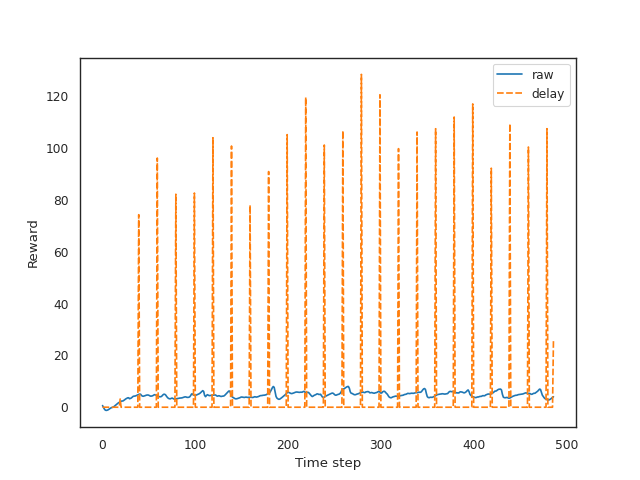
\includegraphics[width=\textwidth]{assets/delay_mode-constant-delay-20_0_delayed.png}

    \caption{Relations between the size of delay interval and policy performance.}
    \label{fig:fig2}
\end{figure}

\subsection{Evaluation on custom simulated datasets}

In order to verify the effectiveness of the reward modification strategy proposed before, we added an artifical task on simulatied environment
in a real-world scenario for verification.

Recommender systems is one of the important scenarios of reinforcement learning applications. In modern recommender systems, the interaction between the users and the recommender system can be abstracted into the interaction between the recommendation agent and the user environment. In the recommender system, it is very difficult to optimize the long-term retention of users,  as retention signal is the 0-1 binary signal obtained at the final moment of a long-term interaction, which is very sparse especially for inactive users. Such retention signals and delay rewards are consistent in definition, therefore, in our experiments, out of user privacy and security requirements, we build a user retention simulation environment based on Google’s open source reinforcement learning recommendation system framework RecSim \cite{ieRecSimConfigurableSimulation2019}.

Datasets for experiments are collected by training an agent interacting with the simulated environment
using Soft Actor-Critic \cite{haarnoja2018soft} from scratch and collecting 1000 trajectories at
4 different levels during training to make the data distribution more complex:
More details on the construction of simulated environment and data collection are available in Appendix \ref{appendix: exp_custom_detials}.

